\chapter{Additional Material For Foundation Models in High-Energy Physics}
\label{app:foundation_models}

In addition to fine-tuning, the performance of frozen pre-trained encoders in the same downstream tasks is investigated.
The results, presented in \Cref{fig:indist_fixed} and \Cref{fig:outdist_fixed}, demonstrate that these backbones provide a feature-rich latent space.

\begin{figure}[h!]
    \centering
    \begin{subfigure}{0.32\linewidth}
        \centering
        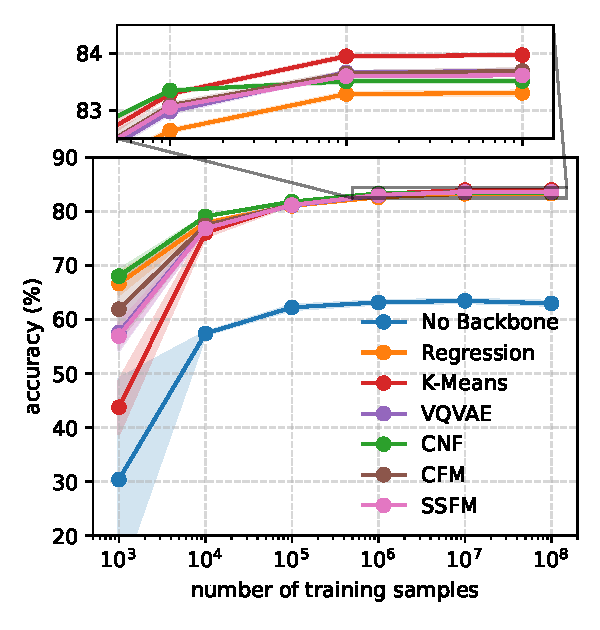
\includegraphics[width=\linewidth]{Figures/foundation_models/mpm2/final/jetclass_frozen.pdf}
        \caption{}
        \label{fig:jetclass_fixed}
    \end{subfigure}
    \begin{subfigure}[b]{0.32\textwidth}
        \centering
        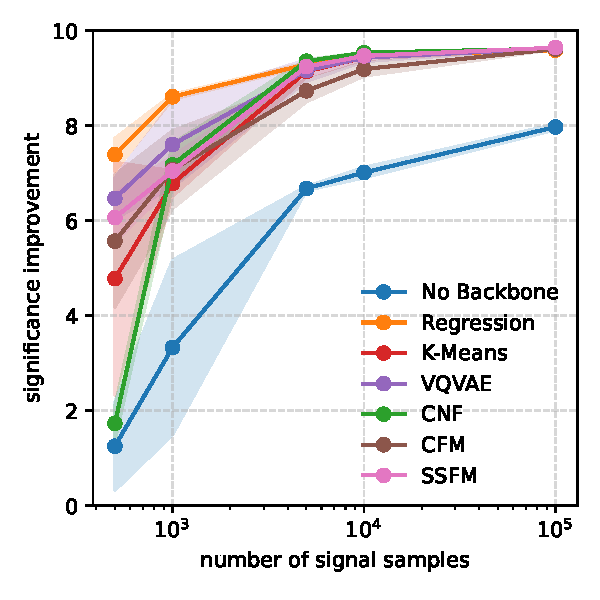
\includegraphics[width=\linewidth]{Figures/foundation_models/mpm2/final/cwola_frozen.pdf}
        \caption{}
        \label{fig:cwola_fixed}
    \end{subfigure}
    \caption{The in-distribution performance of the fixed-backbone models on the JetClass dataset. \subref{fig:jetclass_fixed} shows the accuracy using standard supervised classification as a function of the dataset size.  \subref{fig:cwola_fixed} shows the significance-improvement of the models trained in a CWoLa setting as a function of the number of signal samples in the dataset.}
    \label{fig:indist_fixed}
\end{figure}

\begin{figure}[h!]
    \centering
    \begin{subfigure}{0.32\linewidth}
        \centering
        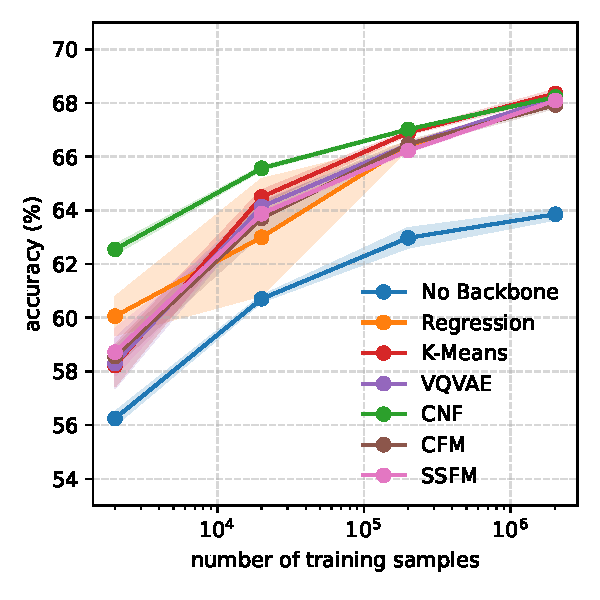
\includegraphics[width=\linewidth]{Figures/foundation_models/mpm2/final/btag_frozen.pdf}
        \caption{}
        \label{fig:btag_frozen}
    \end{subfigure}
    \begin{subfigure}[b]{0.32\textwidth}
        \centering
        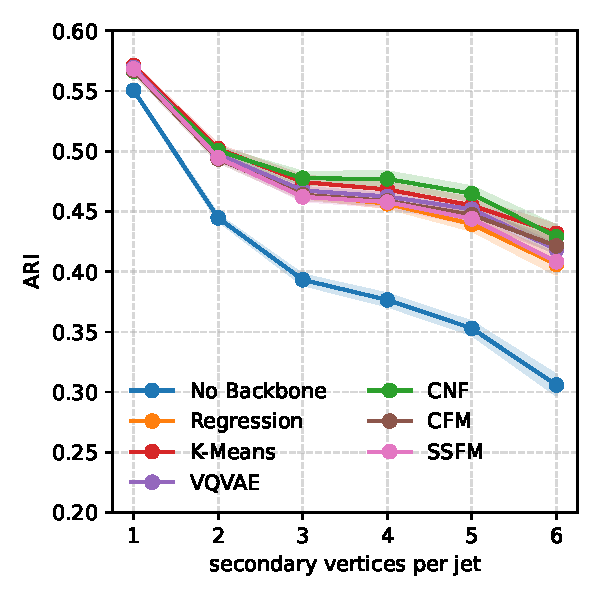
\includegraphics[width=\linewidth]{Figures/foundation_models/mpm2/final/vtx_frozen_ari.pdf}
        \caption{}
        \label{fig:vtx_frozen_ari}
    \end{subfigure}
    \begin{subfigure}[b]{0.32\textwidth}
        \centering
        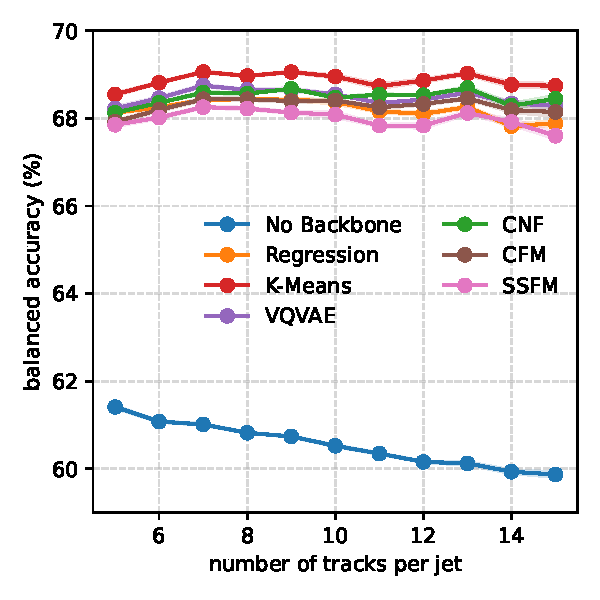
\includegraphics[width=\linewidth]{Figures/foundation_models/mpm2/final/trk_frozen.pdf}
        \caption{}
        \label{fig:trk_frozen}
    \end{subfigure}
    \caption{The performance of the fixed backbone models on the BTag dataset. \subref{fig:btag_frozen} shows the supervised jet classifier accuracy versus the number of samples used in fine-tuning.
        \subref{fig:vtx_frozen_ari} shows the ARI score for the segmentation task versus the number of secondary vertices within each jet.  \subref{fig:trk_frozen} shows the balanced accuracy for the track identification task as a function of the number of tracks in each jet.}
    \label{fig:outdist_fixed}
\end{figure}

Qualitative results of various continuous reconstructions used by MPMv2 tasks are shown in \Cref{fig:reconstruction}.
Three jets are randomly selected from the JetClass dataset, 40\% masking is applied, and each backbone is tasked with reconstructing the dropped constituent features.
Zero-padded impact parameters for neutral particles are not plotted.
For the regression backbone, direct feature predictions are needed.
Reconstruction with the K-Means backbone involves sampling under the discrete distribution of centroid probabilities.
The CNF and CFM backbone allow sampling under the normalizing flow, but the CFM does require numerical integration.
The Regression predictions frequently collapse towards the centre of the distribution.
This is most apparent in the $\Delta \eta$ distribution of Jet-1, which exhibits a bi-modal distribution indicative of a dual-prong jet.
While other methods successfully reconstruct this bi-modality, the Regression backbone merely predicts the mean.
This lack of diversity might explain why the Regression backbone requires a large decoder to perform well.
There is little per-particle information in the space right before the linear layer.

\begin{figure}[h]
    \centering
    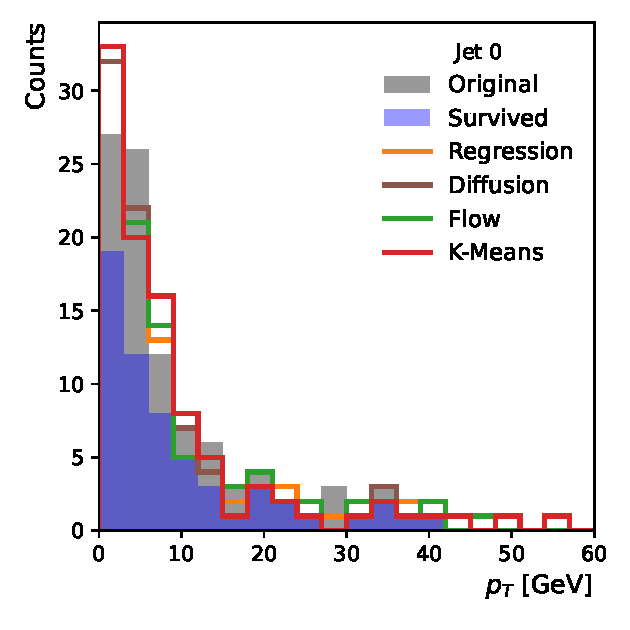
\includegraphics[width=0.32\linewidth]{Figures/foundation_models/mpm2/reconstruction_plots/jet_0_0.pdf}
    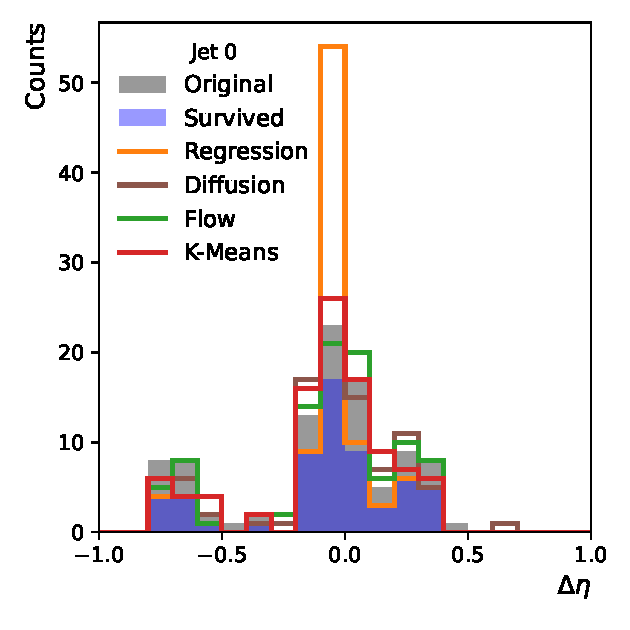
\includegraphics[width=0.32\linewidth]{Figures/foundation_models/mpm2/reconstruction_plots/jet_0_1.pdf}
    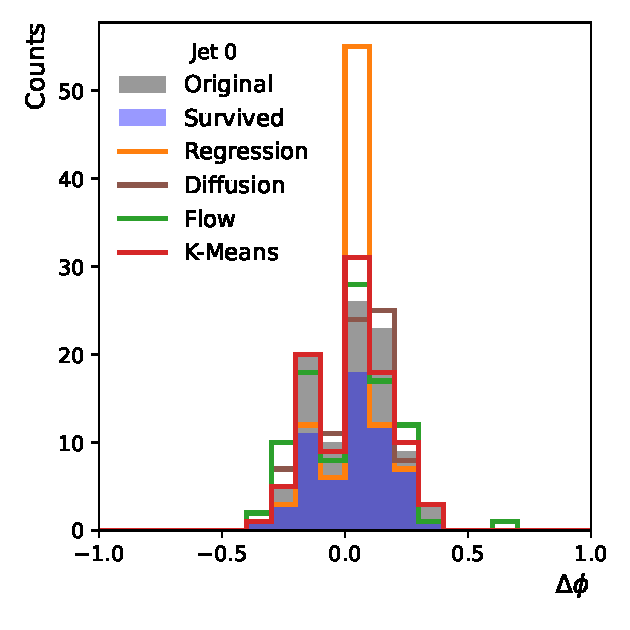
\includegraphics[width=0.32\linewidth]{Figures/foundation_models/mpm2/reconstruction_plots/jet_0_2.pdf}
    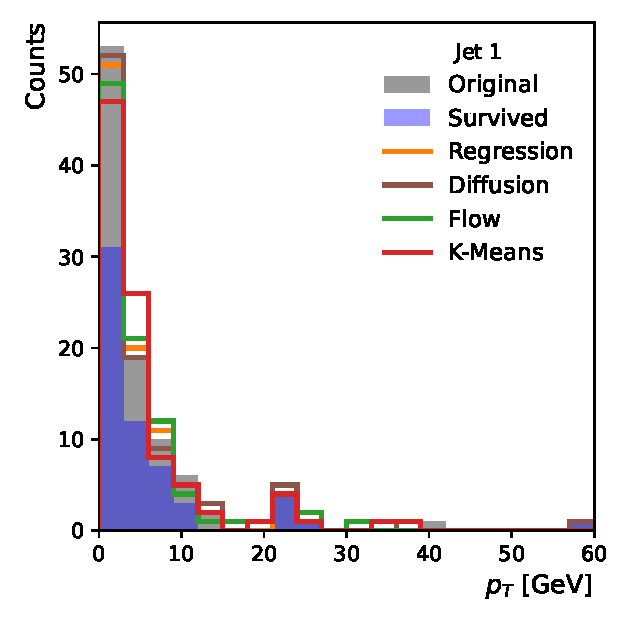
\includegraphics[width=0.32\linewidth]{Figures/foundation_models/mpm2/reconstruction_plots/jet_1_0.pdf}
    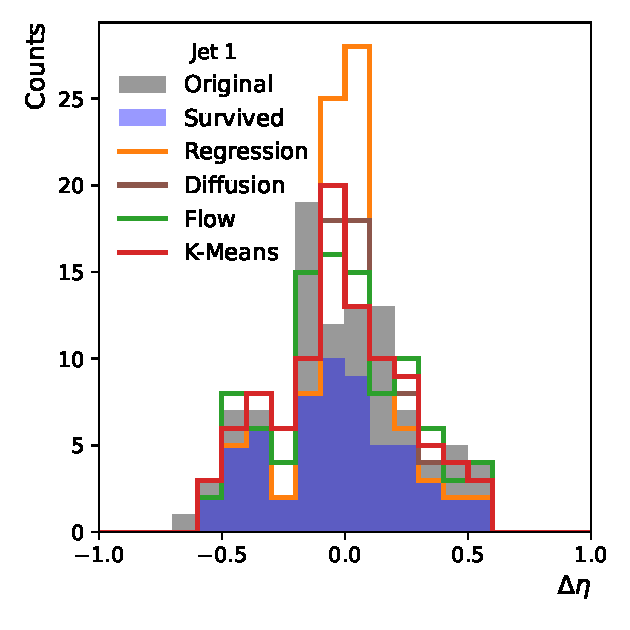
\includegraphics[width=0.32\linewidth]{Figures/foundation_models/mpm2/reconstruction_plots/jet_1_1.pdf}
    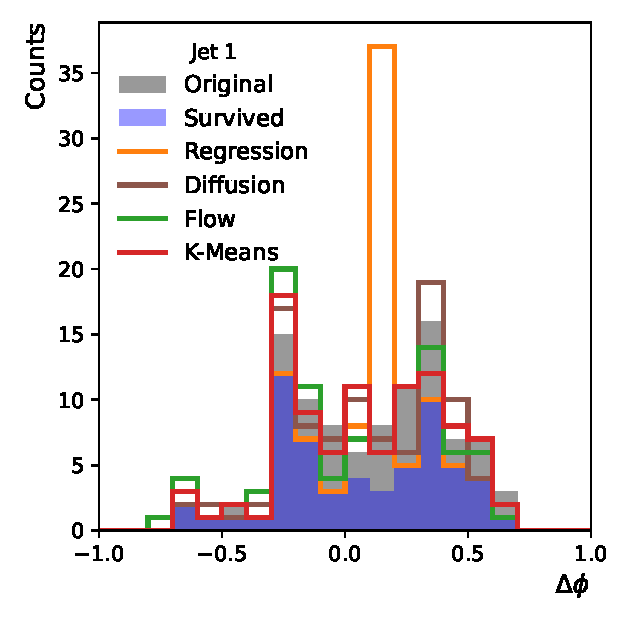
\includegraphics[width=0.32\linewidth]{Figures/foundation_models/mpm2/reconstruction_plots/jet_1_2.pdf}
    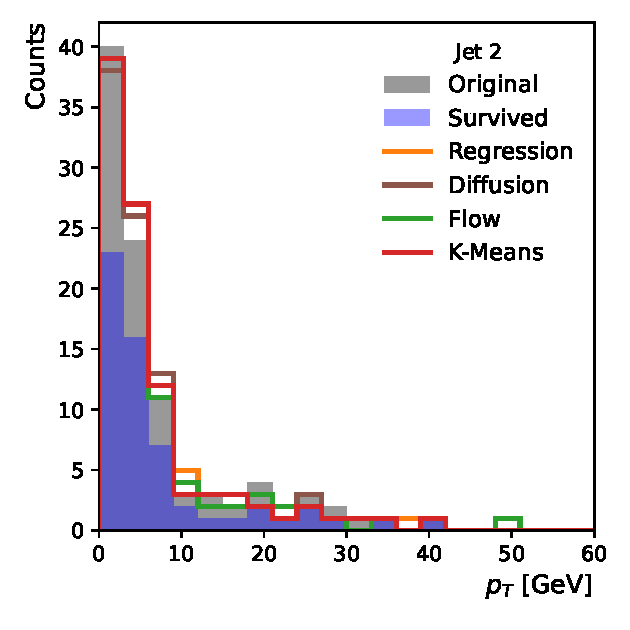
\includegraphics[width=0.32\linewidth]{Figures/foundation_models/mpm2/reconstruction_plots/jet_2_0.pdf}
    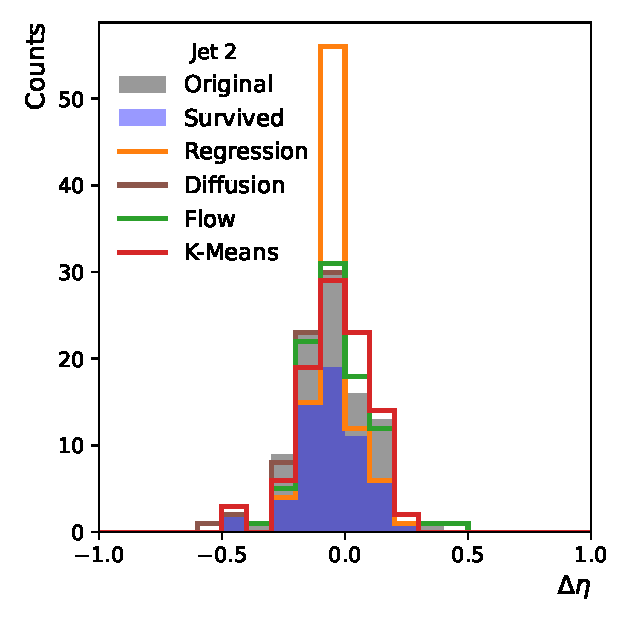
\includegraphics[width=0.32\linewidth]{Figures/foundation_models/mpm2/reconstruction_plots/jet_2_1.pdf}
    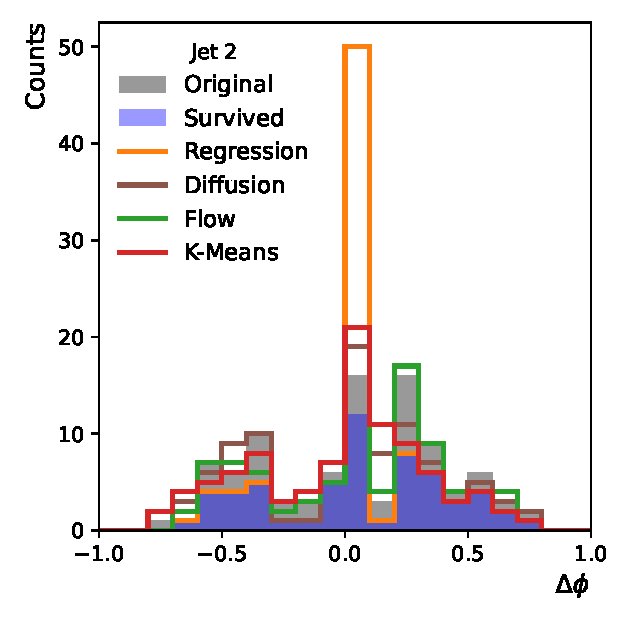
\includegraphics[width=0.32\linewidth]{Figures/foundation_models/mpm2/reconstruction_plots/jet_2_2.pdf}
    \caption{The figure displays three randomly selected jets (rows) from the JetClass dataset, with their $(\pt, \Delta \eta, \Delta \phi)$ distributions plotted (columns). Grey shading indicates the original jet distributions, while blue shading represents the distributions after 40\% of the constituents were dropped. Coloured lines illustrate the reconstructed jets using various methods. The optimal reconstruction would ideally align with the original grey distribution.}
    \label{fig:reconstruction}
\end{figure}
